
\documentclass[journal,transmag]{IEEEtran}
\hyphenation{op-tical net-works semi-conduc-tor}

\usepackage{enumitem}

% *** GRAPHICS RELATED PACKAGES ***
%
\ifCLASSINFOpdf
   \usepackage[pdftex]{graphicx}
  % declare the path(s) where your graphic files are
  % \graphicspath{{../pdf/}{../jpeg/}}
  % and their extensions so you won't have to specify these with
  % every instance of \includegraphics
  % \DeclareGraphicsExtensions{.pdf,.jpeg,.png}
\else
  % or other class option (dvipsone, dvipdf, if not using dvips). graphicx
  % will default to the driver specified in the system graphics.cfg if no
  % driver is specified.
  % \usepackage[dvips]{graphicx}
  % declare the path(s) where your graphic files are
  % \graphicspath{{../eps/}}
  % and their extensions so you won't have to specify these with
  % every instance of \includegraphics
  % \DeclareGraphicsExtensions{.eps}
\fi
% graphicx was written by David Carlisle and Sebastian Rahtz. It is
% required if you want graphics, photos, etc. graphicx.sty is already
% installed on most LaTeX systems. The latest version and documentation
% can be obtained at: 
% http://www.ctan.org/pkg/graphicx
% Another good source of documentation is "Using Imported Graphics in
% LaTeX2e" by Keith Reckdahl which can be found at:
% http://www.ctan.org/pkg/epslatex
%
% latex, and pdflatex in dvi mode, support graphics in encapsulated
% postscript (.eps) format. pdflatex in pdf mode supports graphics
% in .pdf, .jpeg, .png and .mps (metapost) formats. Users should ensure
% that all non-photo figures use a vector format (.eps, .pdf, .mps) and
% not a bitmapped formats (.jpeg, .png). The IEEE frowns on bitmapped formats
% which can result in "jaggedy"/blurry rendering of lines and letters as
% well as large increases in file sizes.
%
% You can find documentation about the pdfTeX application at:
% http://www.tug.org/applications/pdftex





\begin{document}

\title{\textsc{TORRICELLI}}

\author{
\IEEEauthorblockN{David S. Castro , William A. Gómez,  Ana M. Niño, Laura V. Pachón , Juliana Ramos y Luis A. Cañón,}
\IEEEauthorblockA{Pontificia Universidad Javeriana, Bogotá, Colombia}
\IEEEauthorblockA{Informe de laboratorio Teorema Torricelli }
\IEEEauthorblockA{Grupo I}

}
% The paper headers
\markboth{Torricelli. Septiembre 9~2021}%
{Shell \MakeLowercase{\textit{et al.}}: Bare Demo of IEEEtran.cls for IEEE Transactions on Magnetics Journals}
\IEEEtitleabstractindextext{%

	\begin{abstract}
	Torricelli's principle is an application of Bernoulli's equation where we measure the flow of a liquid inside a container through a small hole under the effects of gravity. In this laboratory we worked with a jar that had eight holes which were covered by a piece of wood that prevented the fluid that was placed inside it from leaving the container. The laboratory practice consists of two experiments, in the first one a quantity of volume of water was placed (this quantity was chosen by the members of the group) and each one of the wooden sticks of the buildings was taken out and measured through a rule the distance the fluid reached; the other consisted of choosing an initial quantity of water and taking a different height (this height is less than the initial quantity of water), one of the "plugs" would be removed and the time it took for the fluid to reach the defined height. 
	\end{abstract}
	\begin{IEEEkeywords}
	Torricelli's theorem, Principle of continuity, Bernoulli's equation, Flows, Ideal fluids, Torricelli's montage, Pressure, Density
	\end{IEEEkeywords}}


\maketitle
\IEEEdisplaynontitleabstractindextext
\IEEEpeerreviewmaketitle


\section{Resumen}
El principio de Torricelli es una aplicación de la ecuación de Bernoulli donde medimos el flujo de un líquido dentro de un recipiente a través de un pequeño orificio bajo los efectos de la gravedad. 

En este laboratorio se trabajó con un tarro que contaba con ocho orificios los cuales estaban tapados por un pedazo de madera que impedía que el fluido que se colocara dentro saliera del recipiente. La práctica de laboratorio consta de dos experimentos, en el primero se colocaba una cantidad de volumen de agua (esta cantidad era elegida por los integrantes del grupo) e ir sacando cada uno de los palos de madera de los edificios y medir a través de una regla la distancia que el fluido alcanzaba; el otro, consistía en elegir una cantidad de agua inicial y tomar una altura diferente (esta altura es menor a la cantidad de agua inicial), se quitaba uno de los “tapones” y se mediría el tiempo que tardaba el fluido en llegar a la altura definida.


\section{Introduction}
	
	La siguiente practica de laboratorio se realiza con el propósito de evaluar los principios de conservación de un fluido incompresible ideal en movimiento donde se pueden evidenciar mediante el montaje con los siguientes materiales. 
	
	\begin{enumerate}
	
  \item Vaso de precipitado: Se utilizó para transportar agua
			\begin{figure}[!h]
		\center
		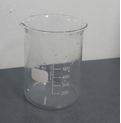
\includegraphics[width=3.5cm]{imagen1.png}
		\caption{Vaso de Precipitado}
		\label{1}
		\end{figure}
  \item Jarra con tapones: Montaje que ilustra el Teorema de Torricelli.  Tiene huecos con tapones cada 3 centimetros.
			 \begin{figure}[!h]
		\center
		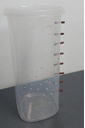
\includegraphics[width=2cm]{imagen2.png}
		\caption{Montaje de Torricelli}
		\label{2}
		\end{figure}
  \item Base: Se utilizo una base de vidrio para registrar las medidas de alcance del agua que sale por los orificios.
			 \begin{figure}[!h]
		\center
		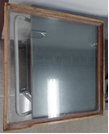
\includegraphics[width=2.5cm]{imagen3.png}
		\caption{Base de vidrio}
		\label{3}
		\end{figure}
 \item Cronometro: El coronometro utilizado para medir el tiempo de vaciado.
				 \begin{figure}[!h]
			\center
			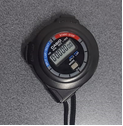
\includegraphics[width=2.5cm]{imagen4.png}
			\caption{Cronómetro}
			\label{4}
			\end{figure}
\item Regla: Se utilizó una regla plastica común, la cual se ubico sobre la base de vidrio.
		 \begin{figure}[!h]
		\center
		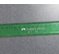
\includegraphics[width=2cm]{imagen5.png}
		\caption{Regla plástica}
		\label{5}
		\end{figure}

	\end{enumerate}
	En primera instancia para el montaje de este laboratorio debemos tener claro que se deben realizar dos actividades en este. Primero hacemos el montaje con la intención de ver cuál es el alcance máximo con respecto a una altura, para ello utilizamos la jarra cuadrada llena de agua a una altura de 3 cm por encima del primer tapón de arriba hacia abajo, posteriormente la ubicamos en la base para que el agua que se libere no se riegue y se pueda reutilizar. 

Después de tener la jarra llena hasta la altura especificada, se van a quitar los tapones que tiene el tarro para dejar liberar el agua en su interior y con una regla que estará en la base se intenta determinar con la mayor exactitud posible cuál es el alcance que tiene el chorro de agua cuando se libera el tapón, es necesario que por cada tapón se tome la medida tres veces para tener un resultado más exacto posible. 

En la segunda parte de la practica vamos a identificar el tiempo de vaciado de un volumen determinado a través de cada uno de los tapones exceptuando el primer tapón de arriba hacia abajo, para poder tomar la medida utilizamos el cronometro y por cada tapón se toma el tiempo de vaciado tres veces. Además, se calculó la cantidad de volumen que se iba a vaciar con la ayuda de una probeta. 

Por último, con los datos recolectados se calculan los errores, la velocidad con los datos obtenidos en la parte que se calculó el tiempo de vaciado para relacionarlos y finalmente se colocan las gráficas para hacer los respectivos análisis y conclusiones. 


\section{Objetivos}

\begin{enumerate}
	
    \item Entender los principios de conservación de un fluido incompresible ideal en movimiento. 
    
    \item Aplicar la ecuación de continuidad y la ecuación de Bernoulli para resolver problemas de hidrodinámica.

	\end{enumerate}
%%%%%%%%%%%%%%%%%%%%%%%%%%MARCO TEÓRICO
\section{Marco Teórico}

 El teorema o principio de Torricelli o principio de Torricelli es una aplicación del principio de Bernoulli y estudia el flujo de un líquido contenido en un recipiente, a través de un pequeño orificio, bajo la acción de la gravedad.  

A partir del teorema de Torricelli se puede calcular el caudal de salida de un líquido por un orificio. “la velocidad de un líquido en una vasija abierta, por un orificio, es la que tendría un cuerpo cualquiera, cayendo libremente en el vacío desde el nivel del líquido hasta el centro de gravedad del orificio”
 
 \begin{figure}[!h]
\center
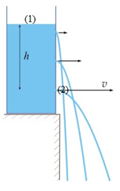
\includegraphics[width=3.5cm]{imagen7.png}
\caption{Diagrama: Montaje-Teorema de Torricelli}
\label{6}
\end{figure}

Aplicando la ecuación de Bernoulli en los puntos (1) y (2) de la Figura \ref{6} siguiente se tiene: 
 
  \begin{figure}[!h] 
\center
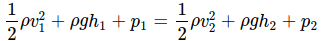
\includegraphics[width=8cm]{imagen8.png}
\caption{Ecuación de Bernoulli}
\label{7}
\end{figure} 

Como la velocidad v1 es muy pequeña se desprecia (=0) y como las presiones p1 y p2  son iguales y corresponden a la presión atmosférica, se cancelan de la Ecuación de Bernoulli; despejando la velocidad en el punto 2, se obtiene: 

  \begin{figure}[!h]
\center
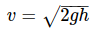
\includegraphics[width=3cm]{imagen9.png}
\caption{Teorema de Torricelli}
\label{8}
\end{figure}
Donde :
\begin{enumerate}[label=(\roman*)]
	
    \item g = a la aceleración de la gravedad
    \item h = a la altura que hay desde el orificio hasta la superficie del líquido 

	\end{enumerate}
\subsection{DEMOSTRACIÓN DEL TEOREMA}
En el teorema de Torricelli y en la fórmula que da la velocidad, supone que las pérdidas por viscosidad son despreciables, al igual que en la caída libre se supone que la fricción debida al aire que circunda al objeto que cae es insignificante. La suposición anterior es razonable en la mayoría de los casos y además implica la conservación de la energía mecánica. 

Para demostrar el teorema, en primer lugar, encontraremos la fórmula de la velocidad para un objeto que se suelta con rapidez inicial cero, desde la misma altura que la superficie líquida en el depósito. 

Se aplicará el principio de la conservación de la energía para obtener la velocidad del objeto que cae justo cuando ha descendido una altura igual a "h", es decir la altura que hay desde la superficie del líquido hasta el orificio. 

Como no hay pérdidas por fricción, es válido aplicar el principio de conservación de la energía mecánica. Supongamos que el objeto que cae tiene masa m y la altura h se mide desde el nivel de salida del líquido. 
\subsection{OBJETO QUE CAE}
Cuando el objeto se suelta desde una altura igual a la de la superficie libre del líquido, su energía es solo potencial gravitatorio, ya que su rapidez es cero y por tanto su energía cinética es nula. La energía potencial Ep está dada por: 
\begin{figure}[!h]
\center
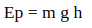
\includegraphics[width=2cm]{imagen10.png}
\caption{Energía mecánica potencial}
\label{f7}
\end{figure}

Cuando va pasando frente al orificio su altura es cero, entonces la energía potencial es cero, por lo que solo tiene energía cinética Ec dada por: 
\begin{figure}[!h]
\center
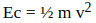
\includegraphics[width=2.2cm]{imagen11.png}
\caption{Energía mecánica cinética}
\label{f7}
\end{figure}


Dado que la energía se conserva Ep = Ec de lo que se obtiene: 
\begin{figure}[!h]
\center
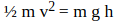
\includegraphics[width=2.6cm]{imagen12.png}
\caption{Conservación de la energía}
\label{f7}
\end{figure}


Despejando la rapidez v se obtiene entonces la fórmula de Torricelli ( Figura \ref{8})

 \subsection{LIQUIDO QUE SALE POR EL ORIFICIO}
 Encontraremos la velocidad de salida del líquido a través del orificio, con el fin de demostrar que coincide con la que recién se calculó para un objeto que cae libremente. Para esto nos basaremos en el principio de Bernoulli, que no es más que la conservación de la energía aplicada a fluidos. 

El principio de Bernoulli se formula así: 

\begin{figure}[!h]
\center
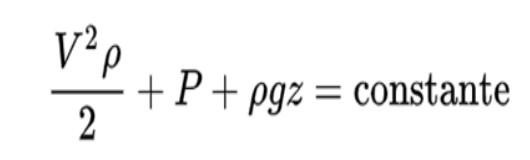
\includegraphics[width=6cm]{imagen13.png}
\caption{Principio de Bernoulli}
\label{12}
\end{figure}
La interpretación de esta fórmula es la siguiente: 
 
 \begin{enumerate}[label=(\roman*)]
	
    \item El primer término representa la energía cinética del fluido por unidad de volumen 
    \item El segundo representa el trabajo realizado por la presión por unidad de área transversal
    \item El tercero representa la energía potencial gravitacional por unidad de volumen de fluido. 
	\end{enumerate}
	
Como partimos de la premisa que se trata de un fluido ideal, en condiciones no turbulentas con velocidades relativamente bajas, entonces es pertinente afirmar que la energía mecánica por unidad de volumen en el fluido es constante en todas las regiones o secciones transversales del mismo. 

En esta fórmula, V es la velocidad del fluido, p es la densidad, P es la presión y z es la posición vertical.
 
 \begin{figure}[!h]
\center
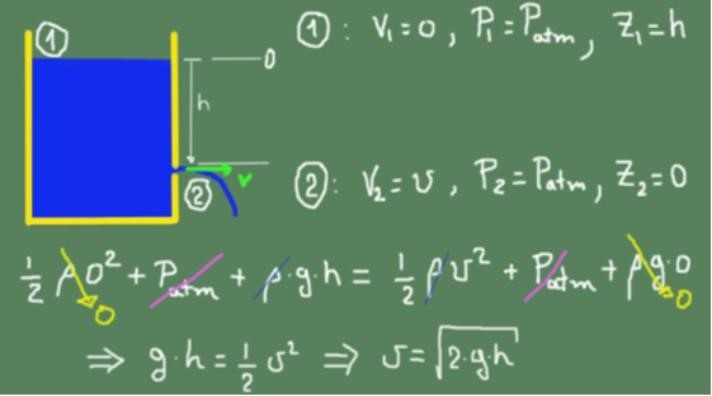
\includegraphics[width=8cm]{imagen14.png}
\caption{Ilustración Principio de Bernoulli-Teorema de Torricelli}
\label{f7}
\end{figure}
 
 Aplicamos la fórmula de Bernoulli en la superficie libre del líquido que denotamos por (1) y en el orificio de salida que denotamos por (2). El nivel de altura cero se ha elegido a ras con el orificio de salida. 

Bajo la premisa que la sección transversal en (1) es mucho mayor que en (2), podemos suponer entonces que la velocidad de descenso del líquido en (1) es prácticamente despreciable. 

Por esto se ha colocado V1=0, la presión a la que está sometida el líquido en (1) es la presión atmosférica y la altura medida desde el orificio es h. 

Para la sección de salida (2) suponemos que la velocidad de salida es v, la presión a la que está sometida el líquido a la salida también es la presión atmosférica y la altura de salida es cero. 

Se sustituyen los valores correspondientes a las secciones (1) y (2) en la fórmula de Bernoulli y se igualan. 
La igualdad tiene validez porque se supone que el fluido es ideal y no hay pérdidas por fricción viscosa. Una vez simplificados todos los términos, se obtiene la velocidad en el orificio de salida. 

El recuadro anterior demuestra que el resultado obtenido es el mismo que el de un objeto que cae libremente:
  \begin{figure}[!h]
\center
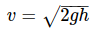
\includegraphics[width=3cm]{imagen9.png}
\caption{Ecuación de Torricelli}
\label{f7}
\end{figure} 
%%%%%%%%%%%%%%%%%%%%%%%%%%METODOLOGIA
\section{Resultados}
\subsection{ALCANCE MÁXIMO}
Para el primer experimento, se tomaron los datos del Alcance Máximo del chorro de agua que salía por agujeros del mismo diámetro a diferentes alturas Hi. Estos datos se repitieron 3 veces (Tabla \ref{T1}). Durante el laboratorio utilizamos una regla plástica normal para medir el alcance máximo, cuyas divisiones en milímetros no fueron utilizadas, pues el tamaño del chorro y su caudal no permitían observar las medidas en milímetros; por esto, se optó por utilizar las divisiones de centímetros para medir el alcance máximo, por lo tanto, la precisión de estas medidas de alcance máximo fue de 0.5 cm. Los datos registrados se muestran en la Tabla \ref{T1}.  Los unidades de los datos estan en el Sistema Internacional de Unidades. 

\begin{table}[!h]
\center
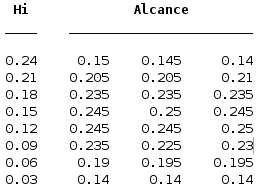
\includegraphics[width=7cm]{tabla1.png}
\caption{Datos registrados: Alcance máximo}
\label{T1}
\end{table}

A continuación, se muestran en la Tabla \ref{T2} con los respectivos datos del promedio, la desviación estándar, la incertidumbre experimental y el error relativo porcentual, de este primer experimento; Se puede decir que los datos fueron medidos con precisión, que realmente es lo que se esperaba pues todos los experimentos fueron muy consistentes entre sus repeticiones. 

\begin{table}[!h]
\center
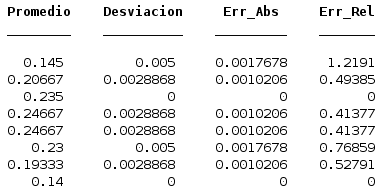
\includegraphics[width=9cm]{tabla2.png}
\caption{Desviación, incertidumbre y error: Alcance máximo}
\label{T2}
\end{table}

Los datos utilizados para realizar la Figura\ref{G1} , del alcance máximo en función de la profundidad de la salida del chorro se muestra en la Tabla \ref{T3}.    
\begin{table}[!h]
\center
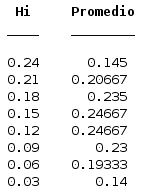
\includegraphics[width=4cm]{tabla3.png}
\caption{Datos utilizados para hacer la Gráfica}
\label{T3}
\end{table}
  \begin{figure}[!h] 
\center
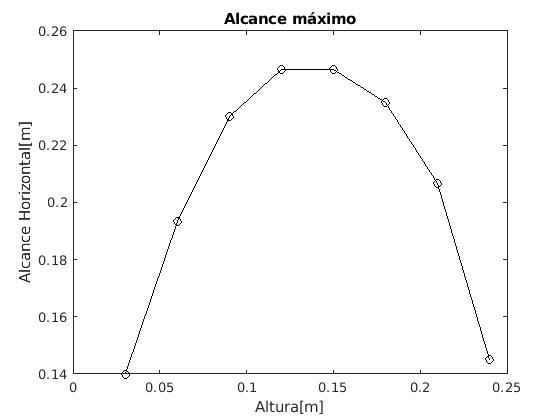
\includegraphics[width=8cm]{grafica1.jpg}
\caption{Alcance del chorro vs Altura del agujero}
\label{G1} 
\end{figure}

   
   
   

\subsection{TIEMPO DE VACIADO}

Por otro lado, en el experimento de medir el tiempo que se demoraba en vaciar un volumen constante desde cada altura diferente, se registraron los datos en la Tabla \ref{T4}, con unidades de metros y segundos respectivamente.  
\begin{table}[!h]
\center
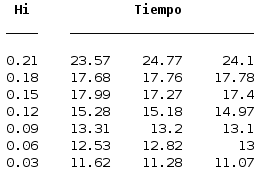
\includegraphics[width=6cm]{tabla4.png}
\caption{Datos registrados: Tiempo de vaciado}
\label{T4}
\end{table}
 
Como ocurrió en los datos tomados en la sección anterior, se obtuvo una buena precisión reflejada en la Tabla \ref{T5} a continuación.   
\begin{table}[!h]
\center
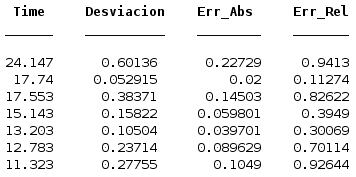
\includegraphics[width=8cm]{tabla5.png}
\caption{Desviacion, incertidumbre y error: Alcance máximo}
\label{T5}
\end{table}

Los datos utilizados para hacer la Figura \ref{G2} se muestran a continuación en la Tabla \ref{T6}. 
\begin{table}[!h]
\center
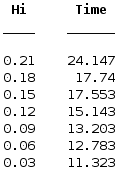
\includegraphics[width=3cm]{tabla6.png}
\caption{Datos utilizados para hacer la Gráfica}
\label{T6}
\end{table}
  \begin{figure}[!h]
\center
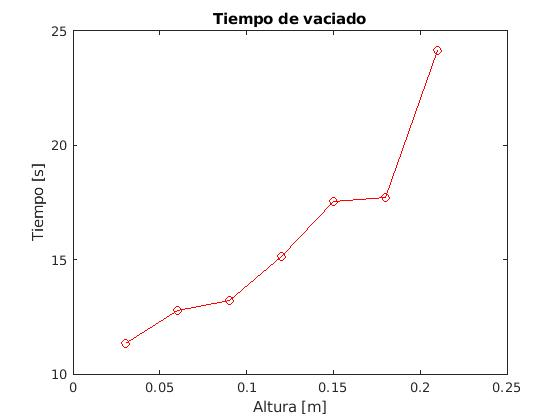
\includegraphics[width=8cm]{grafica2.jpg}
\caption{Tiempo de vaciado vs Altura del agujero}
\label{G2}
\end{figure} 

\subsection{VELOCIDAD DE SALIDA}
Por último, se registraron los datos de la velocidad de salida del agua por cada orificio en la Tabla \ref{T7} haciendo uso de la ecuación de Torricelli. En esta Tabla, la altura Hi inicial corresponde a la medida registrada desde la superficie del líquido, es decir a diferencia de las anteriores Tablas, Hi representa la profundidad y no la altura medida desde la base. 

\begin{table}[!h]
\center
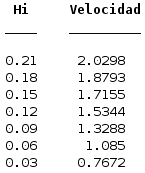
\includegraphics[width=4cm]{tabla7.png}
\caption{Datos utilizados para hacer la Gráfica de Velocidad}
\label{T7}
\end{table}
  \begin{figure}[!h]
\center
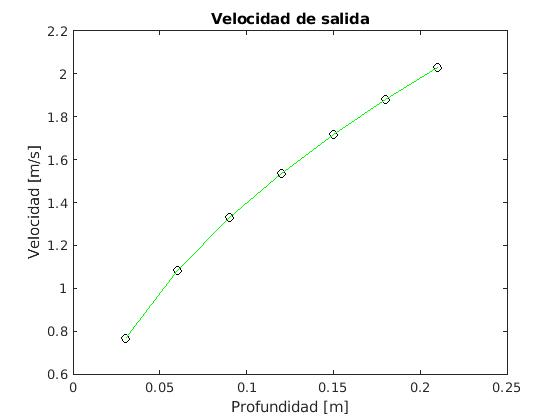
\includegraphics[width=8cm]{grafica3.jpg}
\caption{Velocidad calculada con el Teorema de Torricelli a distintas alturas.}
\label{G3}
\end{figure} 
%%%%%%%%%%%%%%%%%%%%%%%%%%%%%%%%%%%%%%%%%%%%%%%%%%%%RESULTADOS

\section{Análisis de resultados}
\subsection{GRÁFICA 1}
El comportamiento de la gráfica 1 se asemeja al de una parábola cóncava hacia abajo, y por los datos tomados podemos ver que el alcance del fluido no pudo superar los 0.24667 m y que los datos tomados antes y después de llegar al punto máximo de alcance son similares. Esta gráfica muestra que hay un punto máximo de alcance horizontal a una profundidad cerca de los 15 cm desde el fondo, donde a pesar de no tener la máxima velocidad, si se muestra el mayor alcance debido a su posición inicial de salida del chorro. 

Por otro lado, el alcance del fluido está determinado tanto por la altura a la que se encuentra como la proximidad a la zona de impacto, es decir, aunque se tenga una influencia de la presión el efecto no durará lo suficiente para mantener una trayectoria uniforme y marcar una distancia mayor. 
\subsection{GRÁFICA 2}
Podemos ver en la gráfica 2 el claro comportamiento exponencial entre la altura a la que se encuentre la salida del agua y el tiempo que se demorara en vaciarse una misma cantidad de líquido para cada altura. Debido a que a menor profundidad el líquido saldrá con menos velocidad que, a una profundidad mayor, el tiempo de vaciado de un mismo volumen va a depender de la velocidad. Por lo tanto, el tiempo que se demoraría en vaciarse un mismo volumen de agua crece rápidamente al infinito, cerca del punto de la superficie, ya que, por su gran área, y según las consideraciones del modelo de Torricelli, su velocidad de salida es cercana a 0. 
\subsection{GRÁFICA 3}
En primera instancia podemos predecir el comportamiento de la gráfica solo por ver y analizar la fórmula que utilizamos, al tener un radical podemos ver que se comporta de la forma esperada. además, como se esperaba por el teorema de Torricelli, la velocidad del fluido que sale por un orificio a diferentes alturas es comparable con la velocidad de caída libre de un objeto, el cual al estar bajo el efecto de la gravedad experimental, es decir, una aceleración constante, por lo que, a mayor altitud (distancia), la partícula desarrollará una mayor velocidad, es por esto que como se observa en la gráfica , la velocidad aumenta a medida que aumenta la "altura" desde donde la partícula de fluido (superficie del agua) cae y esta llegaría con una velocidad final a la salida del orificio.  

\section{Conclusion}
	
	\begin{enumerate}[label=(\roman*)]
	
    \item Con la práctica de laboratorio podemos justificar el comportamiento de la gráfica de alcance por medio del principio de Bernoulli dado que como dice el mismo principio la relación de velocidad con presión es inversamente proporcional, lo que indica que a medida que la velocidad está aumentando hay menos presión en el fluido haciendo que su alcance comience a disminuir casi en la misma proporción que aumentó. 
    \item La fórmula de velocidad del fluido saliendo por un orificio, se puede asociar con la fórmula de caída libre en mecánica. 
    \item La presión que ejerce el líquido a una mayor altura es menor, provocando que este salga de una forma más lenta, prolongada y a una velocidad menor. Por lo tanto, a mayor altura el tiempo de vaciado es mayor. 
    \item Al realizar varias mediciones en el alcance y el tiempo, se reduce el margen de error aleatorio a causa de la medición tomada por el estudiante, permitiendo tener una baja desviación de los datos con respecto a la media.   

	\end{enumerate}

\appendices


\ifCLASSOPTIONcaptionsoff
  \newpage
\fi


\begin{thebibliography}{1}


 \bibitem{IEEEhowto:Monteria}
  Matemáticas y Física (18 de febrero del 2018). Teorema de Torricelli. Recuperado de: https://matefisicamonteria.blogspot.com/2018/02/teorema-de-torricelli.html 
 \bibitem{IEEEhowto:Monteria}
 Fanny Zapata. (4 de mayo de 2019). Teorema de Torricelli: en qué consiste, fórmulas y ejercicios. Lifeder. Recuperado de: https://www.lifeder.com/teorema-de-torricelli/ 
 \bibitem{IEEEhowto:Monteria}
 Ilustración 6. Probeta. Grupo didacta. Enlace: https://grupodidacta.com/product/cilindro-graduado-o-probeta-100-ml-referencia-ch0345k/  
\end{thebibliography}



\end{document}
